\chapter{Phase 4 - Zero-Shot Shelf Monitoring}
\setcounter{section}{0}
\renewcommand{\thesection}{\arabic{section}}
\label{chap:phase4-zeroshot}

\section{Introduction}
This chapter presents the technical background and implementation work for the retail inventory capabilities within the EYE-D video analytics solution. The work described here corresponds to Phase 4 of the project, which focused on a Zero-Shot Shelf Fullness Detection system. In contrast to previous supervised learning approaches (e.g., forklift detection), this phase leverages advanced Vision-Language Models (VLMs) to detect objects based on natural language prompts without requiring a single annotated bounding box for that specific class. The primary goal is to make zero-shot models work on specific hardware constraints (NPU) for broader use cases, heavily emphasizing ONNX exportation and optimized inference engines customized for users' specific operational conditions.

\section{Zero-Shot Detection Paradigms (SoTA)}

\subsection{Evolution of Detection: Transition from Bounding Box Regression to Semantic Grounding}
The paradigm of computer vision in industrial retail has historically relied on supervised learning, where models are trained to perform bounding box regression on a finite, predefined set of classes. This approach inherently struggles with the dynamic nature of retail environments, where Stock Keeping Units (SKUs) are continuously introduced, removed, or redesigned. Consequently, the field is undergoing a fundamental transition toward semantic grounding. Rather than predicting spatial coordinates tied to an arbitrary integer class ID, semantic grounding aligns visual features with unconstrained textual descriptions. This evolutionary step eliminates the bottleneck of continuous dataset annotation, enabling intelligent systems to generalize to novel objects simply by interpreting natural language queries.

Building upon this foundational shift, the introduction of multi-modal architectures has bridged the gap between natural language processing and computer vision.

\subsection{Vision-Language Models (VLMs)}
Vision-Language Models (VLMs) represent the convergence of linguistic comprehension and visual perception. In traditional pipelines, a model only recognizes patterns it has been explicitly trained to see. Conversely, VLMs utilize a dual-encoder architecture where text prompts (e.g., ``empty shelf'' or ``metal shelving'') are mapped into dense feature vectors using a language encoder. Simultaneously, the image is processed by a vision encoder to extract spatial features. The model then computes the cross-modal similarity between the text embeddings and the visual regions. This interaction allows the system to identify the precise spatial location of an object based solely on its textual description. This capability, known as \textbf{Text-to-Box Grounding}, empowers the system to detect abstract concepts like ``negative space'' without requiring a single annotated bounding box for that specific class \cite{ref:groundingdino}.

With the underlying mechanics of VLMs established, it is necessary to examine the specific architectures deployed in this system to balance accuracy and edge constraints.

\subsection{Open-Vocabulary Detectors}
\textbf{Open-Vocabulary Detection} is the practical application of VLMs, enabling a model to detect any object requested by a user prompt at runtime. To achieve robust performance in edge environments, this system integrates two distinct open-vocabulary architectures: Grounding DINO and YOLO-World. Grounding DINO operates as a high-precision transformer, deeply fusing vision and language features across multiple attention layers to achieve state-of-the-art accuracy in complex semantic queries \cite{ref:groundingdino}. However, this precision demands significant computational resources. To mitigate this, YOLO-World is employed as a highly efficient counterpart. YOLO-World leverages a RepVGG-based backbone combined with a streamlined vision-language path aggregation network, optimizing the architecture for real-time inference and lower memory consumption \cite{ref:yoloworld}.

\begin{table}[h]
\centering
\caption{Comparative Analysis of Open-Vocabulary Detectors for Edge Deployment}
\label{tab:vlm-comparison}
\renewcommand{\arraystretch}{1.2}
\begin{tabular}{|p{0.30\textwidth}|p{0.32\textwidth}|p{0.32\textwidth}|}
\hline
\textbf{Metric} & \textbf{Grounding DINO} & \textbf{YOLO-World} \\
\hline
\textbf{Accuracy (Semantic Precision)} & Extremely High & High \\
\hline
\textbf{Latency (Inference Speed)} & High & Low (Real-Time) \\
\hline
\textbf{Memory Usage (Footprint)} & High (~VRAM intensive) & Low (Optimized for Edge) \\
\hline
\textbf{Primary Use Case} & Complex Text-to-Box Grounding & Resilient, low-latency fallback \\
\hline
\end{tabular}
\end{table}

This comparative dynamic dictates the operational strategy, ensuring that the highest possible accuracy is maintained without compromising system stability.

\subsection{Evaluation Metrics}
Evaluating the performance of a zero-shot system requires adapting traditional metrics to an open-vocabulary context. Without pre-defined classes, accuracy must be quantified based on the spatial alignment of the text prompt to the physical reality of the shelf.

To evaluate the zero-shot detector, the standard Mean Average Precision (mAP) is modified to assess semantic similarity thresholds alongside spatial overlap. The zero-shot mAP is defined as:
\begin{equation}
mAP_{ZS} = \frac{1}{N_{prompts}} \sum_{i=1}^{N_{prompts}} \int_{0}^{1} P_{i}(R) dR
\end{equation}
where $P_{i}(R)$ is the precision-recall curve for a specific textual prompt $i$, evaluated over a set of unseen classes or semantic concepts.

Furthermore, the primary operational output is the \textbf{Fullness Ratio (\%)}, which quantifies the inventory density. Instead of counting individual SKUs, the system leverages ``Negative Space Analysis.'' The ratio is calculated by comparing the detected product area against the total detected empty shelf area:
\begin{equation}
\text{Fullness Ratio (\%)} = \left( \frac{\sum \text{Area}_{products}}{\sum \text{Area}_{products} + \sum \text{Area}_{empty\_voids}} \right) \times 100
\end{equation}

These mathematical foundations drive the logic of the operational pipeline detailed in the subsequent section.

\section{The 10-Step Fullness Pipeline (Design)}

\subsection{Conceptual Architecture}
The conceptual architecture of Phase 3 is anchored in the theory of \textbf{Negative Space}. In highly variable retail environments, tracking the presence of every unique product is computationally and logistically prohibitive. Negative Space theory inverts this problem: the system focuses on detecting the structural substrate of the shelf and the explicit absence of products (voids). By quantifying the empty spaces against the known physical boundaries of the shelving unit, the system deduces inventory levels deterministically, rendering it immune to SKU variation.

To execute this conceptual approach reliably on edge hardware, a structured and resilient pipeline is required.

\subsection{The Resilient Workflow}

\textbf{Phase A: Validation}
\begin{enumerate}
    \item \textbf{Frame Capture:} The industrial camera provides a raw RTSP video frame.
    \item \textbf{Quality Assessment:} The frame undergoes a rapid check for exposure, blur, and lighting conditions.
    \item \textbf{Shelf ROI Extraction:} The primary Region of Interest (ROI) containing the shelving unit is isolated.
    \item \textbf{Perspective Correction:} Homography transformations correct lens distortion, aligning the shelf to a flat 2D plane for accurate spatial calculations.
\end{enumerate}

\textbf{Phase B: Detection}
\begin{enumerate}
    \setcounter{enumi}{4}
    \item \textbf{Prompt Injection:} The system dynamically injects text prompts (e.g., ``products'', ``empty shelf void'').
    \item \textbf{Dual-Polarity Inference:} The VLM executes simultaneously to detect both the positive space (products) and the negative space (voids).
    \item \textbf{3D Confidence Vector Validation:} Each detection is validated using three distinct metrics:
    \begin{itemize}
        \item \textit{Classification Score:} The semantic probability that the detected region matches the text prompt.
        \item \textit{Detection Probability:} The spatial confidence (Intersection over Union) of the bounding box.
        \item \textit{Context Relevance:} A logical check ensuring the detection makes physical sense (e.g., a void cannot overlap entirely with a product).
    \end{itemize}
\end{enumerate}

\textbf{Phase C: Quantification}
\begin{enumerate}
    \setcounter{enumi}{7}
    \item \textbf{Area Aggregation:} The total pixel area of validated products and empty voids is computed.
    \item \textbf{Fullness \% Calculation:} The system calculates the Fullness Ratio using the mathematical formula.
    \item \textbf{Tier Classification:} The final percentage is mapped to an operational action tier (Tier 1: >80\% Optimal, Tier 2: 50-80\% Monitor, Tier 3: 20-50\% Restock, Tier 4: <20\% Critical).
\end{enumerate}

This sequential processing ensures deterministic outputs, but deploying such a pipeline on edge NPUs necessitates strict fault-tolerance mechanisms.

\subsection{Fault-Tolerance Logic and NPU Optimization}
Operating massive VLMs in an air-gapped, edge-constrained environment poses significant thermal and memory challenges. To ensure uninterrupted operation without cloud connectivity, the system utilizes \textbf{INT8 quantization} for Grounding DINO and \textbf{FP16 quantization} for YOLO-World via ONNX export \cite{ref:onnx}, drastically reducing their memory footprints. 

Despite quantization, sudden spikes in scene complexity can cause Out of Memory (OOM) errors on the NPU. To combat this, the architecture features a \textbf{Hot-Swap Fallback Protocol}. An NPU Memory Watchdog continuously monitors VRAM utilization. Under normal conditions, the high-precision Grounding DINO (INT8) acts as the primary inference engine. If the watchdog detects an impending memory threshold breach, it instantly suspends the primary model and routes the image input to the secondary YOLO-World (FP16) engine. This resilient decision-tree logic guarantees that the pipeline never halts, maintaining continuous shelf monitoring under all hardware conditions.

\begin{figure}[h]
\centering
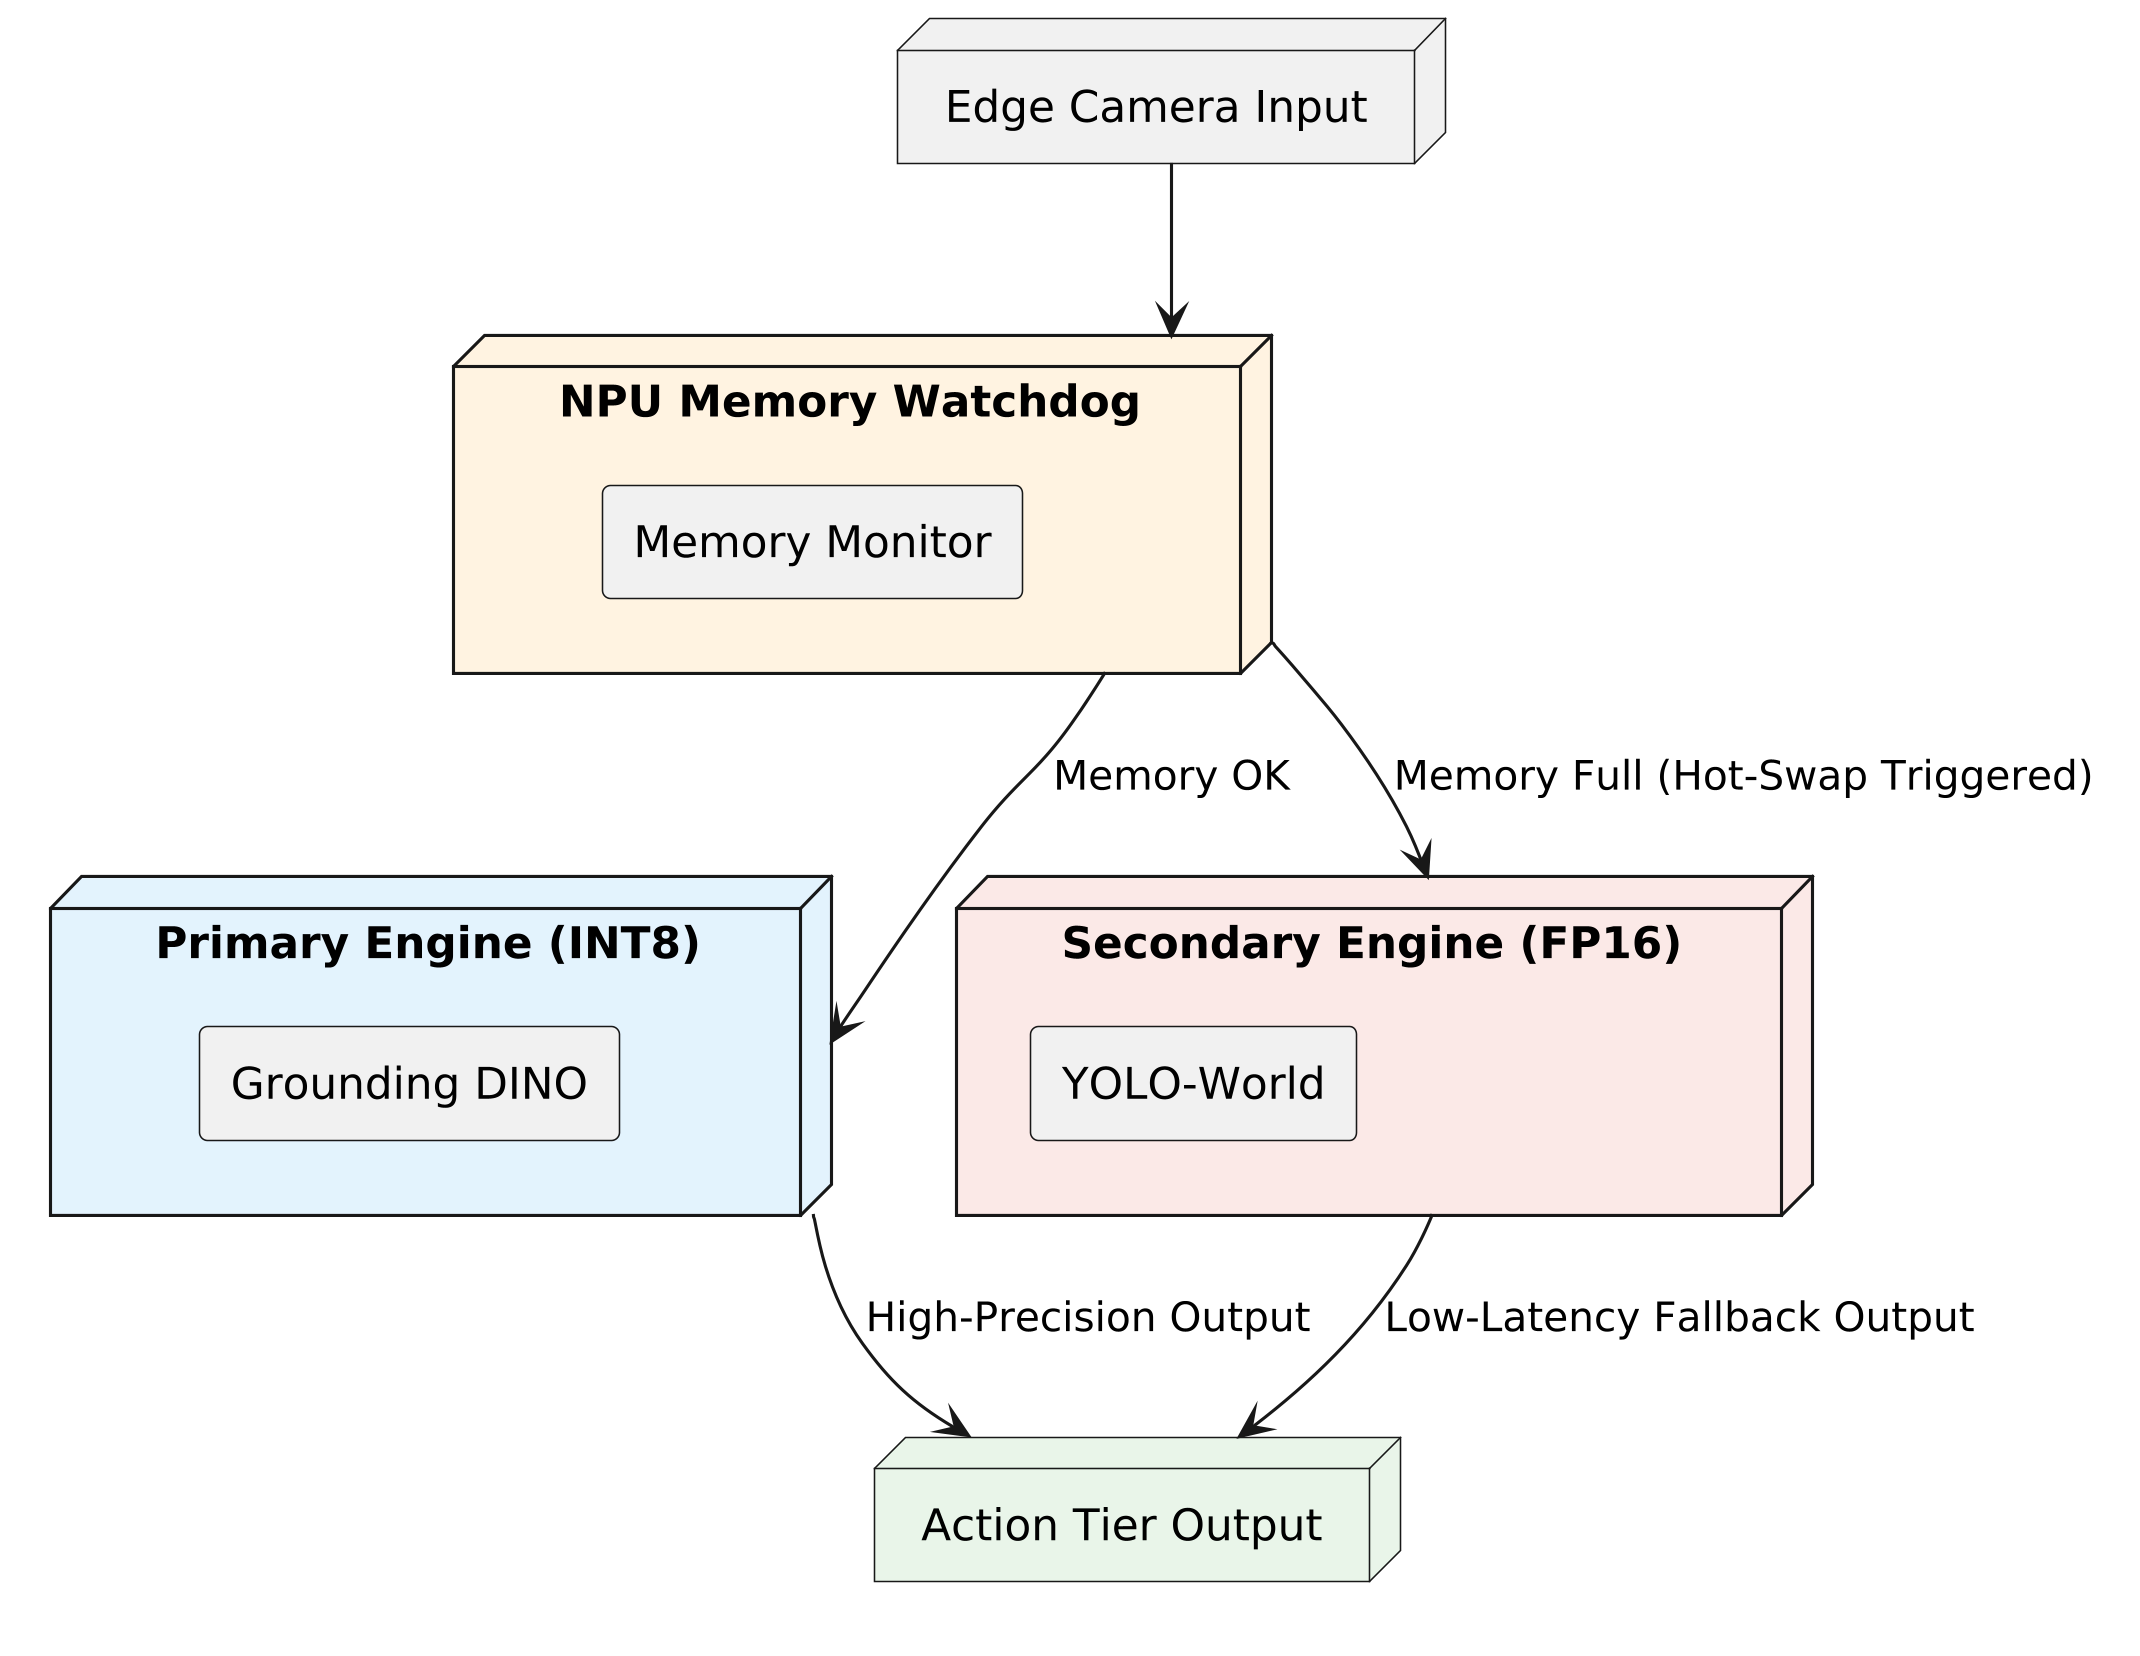
\includegraphics[width=\textwidth]{images/fallback_new.png}
\caption{Multi-model resilient fallback architecture for NPU-constrained deployment.}
\label{fig:fallback-architecture}
\end{figure}

\section{Implementation Output and Negative Space Detection}
The implementation of this zero-shot architecture successfully abstracts away the complexities of SKU-level tracking. Figures \ref{fig:shelf-full}, \ref{fig:shelf-half-empty}, and \ref{fig:shelf-empty} demonstrate the visual output of the zero-shot model detecting shelf voids (negative space) against product space across different inventory levels, verifying the operational success of the models after being exported to ONNX and deployed.

\begin{figure}[H]
\centering
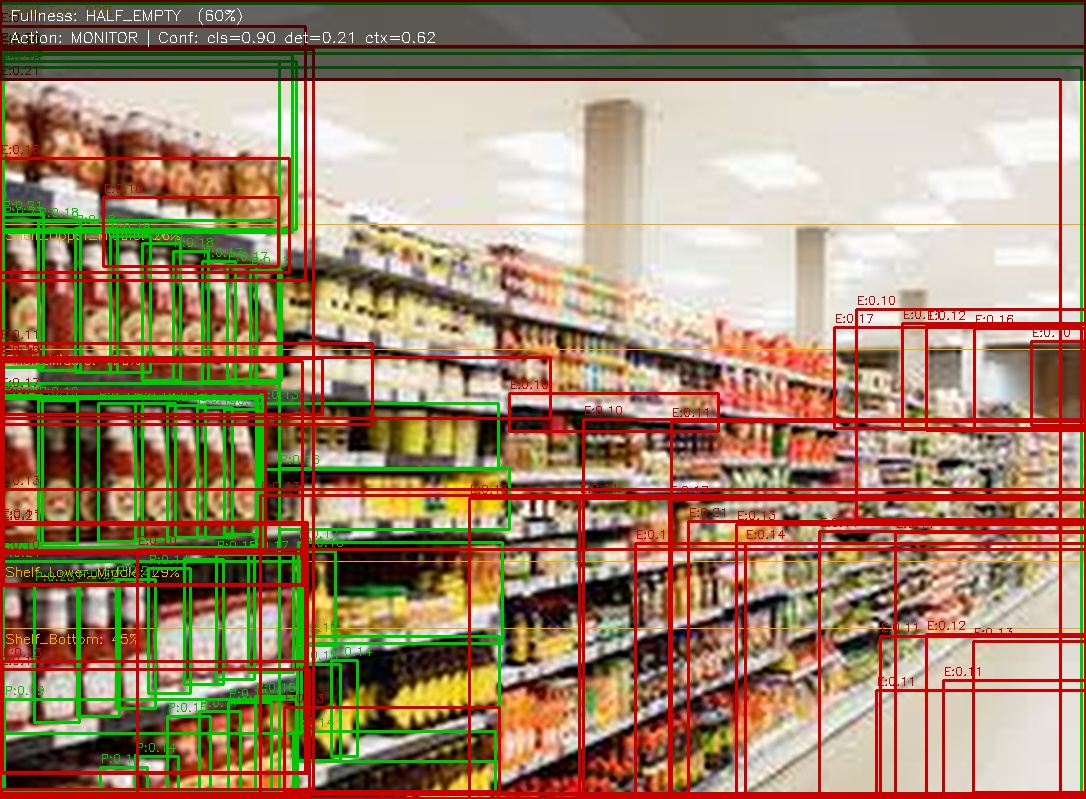
\includegraphics[width=0.75\textwidth]{images/shelf1_annotated.jpg}
\caption{Visual example of Negative Space detection identifying shelf voids on a fully stocked shelf.}
\label{fig:shelf-full}
\end{figure}

\begin{figure}[H]
\centering
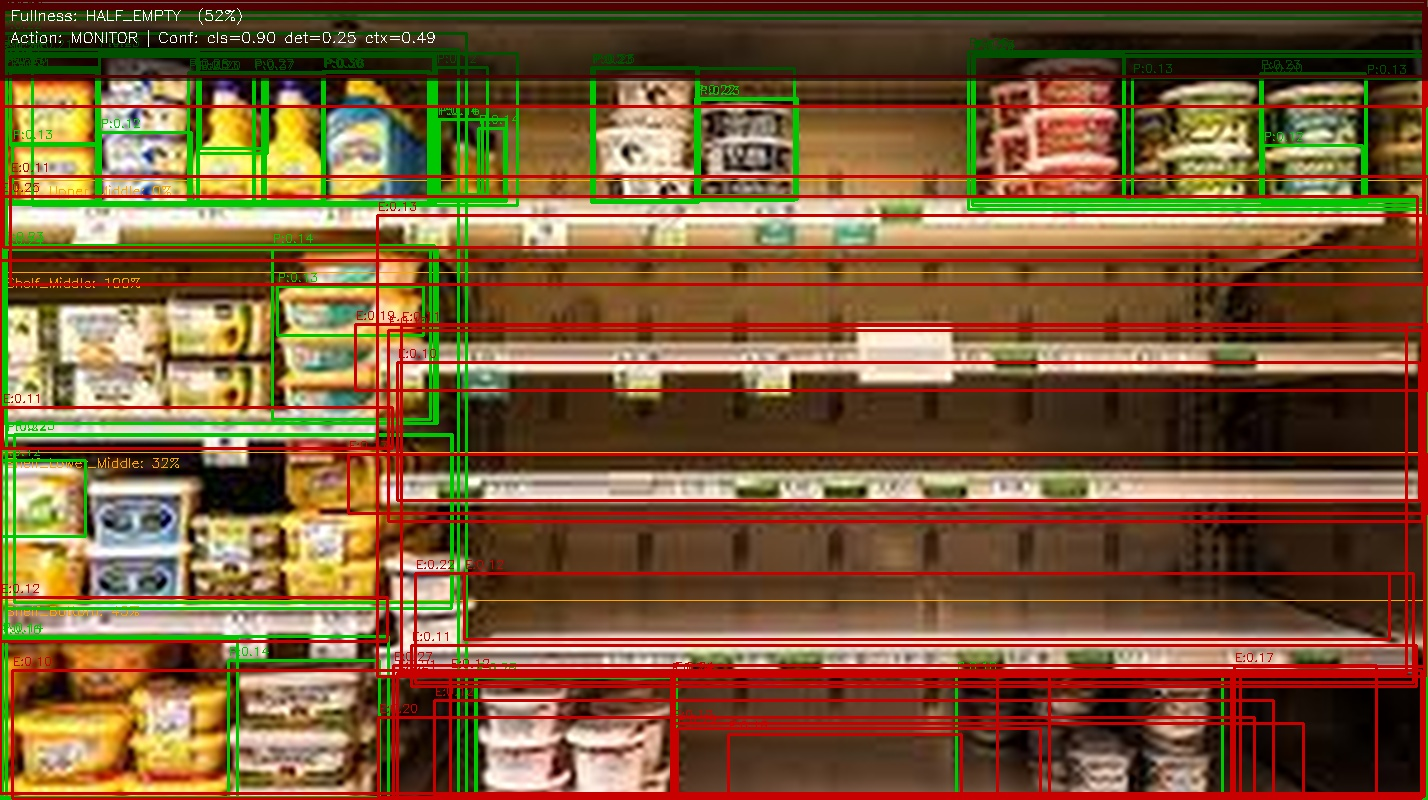
\includegraphics[width=0.75\textwidth]{images/shelf4_annotated.jpg}
\caption{Visual example of Negative Space detection identifying shelf voids on a half-empty shelf.}
\label{fig:shelf-half-empty}
\end{figure}

\begin{figure}[H]
\centering
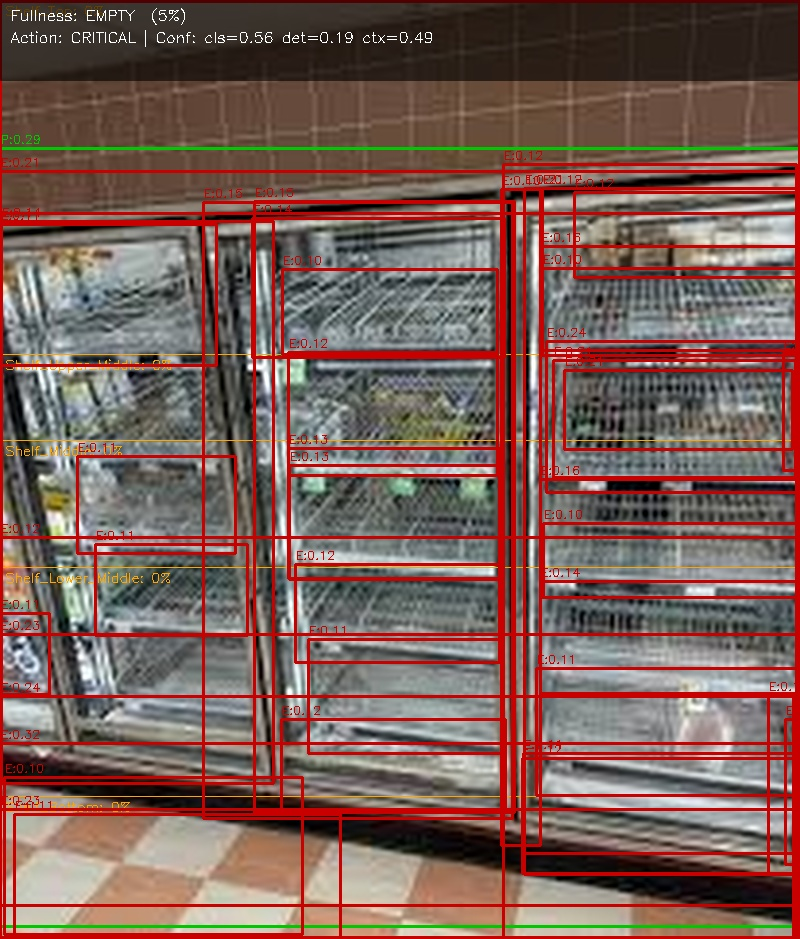
\includegraphics[width=0.75\textwidth]{images/shelf3_annotated.jpg}
\caption{Visual example of Negative Space detection identifying shelf voids on a completely empty shelf.}
\label{fig:shelf-empty}
\end{figure}

\clearpage
\section{Chapter Summary}
By fusing high-accuracy VLMs with robust edge-optimization strategies, the system delivers an air-gapped, fault-tolerant solution capable of real-time inventory monitoring. The resilient fallback mechanism ensures that the theoretical benefits of semantic grounding are practically viable within the strict constraints of industrial NPUs. The most important point of Phase 4 was to verify that the zero-shot model could run effectively on the hardware, proving that clients of the device could easily customize their conditions and dynamically monitor different products using natural language, all without the need for exhaustive data collection or re-training.

Furthermore, this deployment represents the culmination of the project's MLOps lifecycle. To achieve optimal performance on the target NPU, ONNX INT8 quantization was systematically applied to the weights. This process completes the "Full Circle" of the project's engineering methodology: starting from the rigorous data collection and engineering of the 22,607-image dataset (\textbf{Phase 1}), progressing through the supervised fine-tuning and hard-negative mining for safety and logistics (\textbf{Phases 2 \& 3}), and culminating in the NPU optimization and deployment of advanced zero-shot capabilities (\textbf{Phase 4}). This comprehensive approach ensures that all models-whether fine-tuned or open-vocabulary-are deeply aligned with the specific hardware constraints and operational realities of the host organization.



